\documentclass[12pt, a4paper]{article}
\usepackage[utf8]{inputenc}
\usepackage{graphicx}
\usepackage{booktabs}
\usepackage{amsmath}
\usepackage{geometry}
\usepackage{float}

% Page margins
\geometry{left=2.5cm, right=2.5cm, top=2.5cm, bottom=2.5cm}

\title{Methodology and System Structure for Air Quality Prediction}
\author{Author Name}
\date{\today}

\begin{document}

\maketitle

\section{Methodology}

\subsection{System Structure and Architecture}
The air quality prediction system proposed in this study is built upon a \textbf{Stacked Generalization (Ensemble Learning)} architecture. This approach combines the predictions of multiple diverse models, known as ``base-models'' or ``experts,'' which are then fed into a final ``meta-model'' to produce a more robust and accurate final prediction.

The system structure consists of three main hierarchical layers:
\begin{enumerate}
    \item \textbf{Data Acquisition and Preprocessing Layer:} Responsible for gathering both ground-truth and satellite/weather data, cleaning missing entries, and preparing the feature set.
    \item \textbf{Base Model Layer (Ensemble Experts):} Two distinct machine learning models were trained on the primary feature set to generate initial predictions:
    \begin{itemize}
        \item Random Forest Regressor (RF)
        \item XGBoost Regressor (XGB)
    \end{itemize}
    \item \textbf{Meta-Model Layer (Stacking Manager):} A \textbf{Linear Regression} model serves as the stacking manager, trained using the outputs of the two base models as its input features to generate the final, optimized PM2.5 prediction.
\end{enumerate}

\subsection{Data Sources and Collection}
The model development utilized a fused dataset combining ground-truth air quality measurements with corresponding satellite and meteorological variables.

\subsubsection{Ground-Truth Data}
The target variable for prediction is the \textbf{PM2.5 concentration} ($\mu g/m^3$). This data was sourced from a real-time air quality index dataset (CSV), serving as the ground truth for model training.

\subsubsection{Feature Data (Predictor Variables)}
The predictor variables were derived from a fused dataset that combines ground readings with data extracted from the \textbf{Google Earth Engine (GEE)} platform. The final feature set ($X$) includes six key variables:
\begin{itemize}
    \item \textbf{Satellite Data:} Aerosol Optical Depth (AOD).
    \item \textbf{Meteorological Data:} Temperature ($^{\circ}C$), u-component of wind at 10m, and v-component of wind at 10m.
    \item \textbf{Geospatial Data:} Latitude and Longitude.
\end{itemize}

\subsection{Data Preprocessing}
Data preparation was performed to ensure model quality through the following steps:
\begin{enumerate}
    \item \textbf{Missing Value Handling:} Rows with missing ground-truth pollutant averages were removed. Additionally, any rows in the fused dataset missing critical predictor data, specifically AOD or Temperature, were dropped.
    \item \textbf{Feature Standardization:} Raw geospatial coordinate information (JSON strings) was processed to extract and separate latitude and longitude values into distinct floating-point columns.
    \item \textbf{Cleaning:} Rows where coordinate extraction failed were removed to ensure a consistent dataset.
\end{enumerate}

\subsection{Model Training and Evaluation}

\subsubsection{Training Protocol}
The cleaned dataset was partitioned into a \textbf{training set (80\%)} and a \textbf{testing set (20\%)} using a random seed (`random\_state=42`) to ensure reproducibility.

The training process involved two stages:
\begin{enumerate}
    \item \textbf{Base Models:} The Random Forest Regressor and XGBoost Regressor were both trained on the complete training feature set ($\mathbf{X}_{train}$) with `n\_estimators=100`.
    \item \textbf{Meta-Model:} Predictions were generated for the test set using both base models. These predictions ($\text{RF}_{pred}$ and $\text{XGB}_{pred}$) were used as features to train the Linear Regression meta-model against the true target values ($\mathbf{y}_{test}$).
\end{enumerate}

\subsection{Comparative Results (Test Set)}
Model performance was evaluated on the held-out test set using \textbf{R-squared ($R^2$)} and \textbf{Root Mean Squared Error (RMSE)}. The $R^2$ metric indicates the proportion of variance in the dependent variable predictable from the independent variables, while RMSE measures the average magnitude of the error.

Table \ref{tab:results} summarizes the performance of the individual base models compared to the final stacked ensemble.

\begin{table}[H]
    \centering
    \caption{Comparative Performance Metrics on Test Set}
    \label{tab:results}
    \begin{tabular}{lccc}
        \toprule
        \textbf{Model} & \textbf{R-squared ($R^2$)} & \textbf{RMSE ($\mu g/m^3$)} & \textbf{Role} \\
        \midrule
        Random Forest Regressor & 0.5367 & 65.54 & Base Model \\
        XGBoost Regressor & 0.4276 & 72.85 & Base Model \\
        \textbf{Stacked Ensemble Model} & \textbf{0.5592} & -- & \textbf{Final Model} \\
        \bottomrule
    \end{tabular}
\end{table}

The \textbf{Stacked Ensemble Model} achieved the highest $R^2$ score of \textbf{0.5592}, outperforming the Random Forest ($0.5367$) and XGBoost ($0.4276$) base models. This demonstrates that combining the strengths of multiple algorithms via stacking leads to superior predictive accuracy for PM2.5 concentrations.

\section{System Deployment Structure}
To operationalize the proposed methodology, the system is designed as an API endpoint capable of real-time inference. The deployment logic follows this sequence:

\begin{enumerate}
    \item \textbf{Input Collection:} The system accepts user-provided geospatial coordinates (Latitude, Longitude) and the current Aerosol Optical Depth (AOD).
    \item \textbf{Live Data Retrieval:} A real-time weather fetcher retrieves the necessary meteorological parameters (Temperature, U-wind, V-wind) from the OpenWeatherMap API.
    \item \textbf{Feature Integration:} Static inputs and dynamic weather data are aggregated into a single feature vector matching the training schema.
    \item \textbf{Stacked Prediction:} The feature vector is passed through the Random Forest and XGBoost models. Their outputs are fed into the Linear Regression meta-model to compute the final PM2.5 concentration.
    \item \textbf{Classification:} The predicted concentration is mapped to the official Indian AQI categories (e.g., Good, Moderate, Poor) and returned as a JSON response.
\end{enumerate}

\end

\documentclass[conference]{IEEEtran}
\IEEEoverridecommandlockouts
% The preceding line is only needed to identify funding in the first footnote. If that is unneeded, please comment it out.

\usepackage{cite}
\usepackage{amsmath,amssymb,amsfonts}
\usepackage{algorithmic}
\usepackage{graphicx}
\usepackage{textcomp}
\usepackage{xcolor}
% Make sure float is included for table placement if needed later,
% though figure* handles its own placement.
\usepackage{float}
\usepackage{booktabs} % For professional looking tables

\def\BibTeX{{\rm B\kern-.05em{\sc i\kern-.025em b}\kern-.08em
    T\kern-.1667em\lower.7ex\hbox{E}\kern-.125emX}}
\begin{document}

\title{A Stacked Ensemble Learning Approach for Hyper-Local PM2.5 Prediction Using Satellite AOD and Meteorological Data}

\author{\IEEEauthorblockN{1\textsuperscript{st} Md. Masum Billah}
\IEEEauthorblockA{\textit{Computer Science and Engineering (of Aff.)} \\
\textit{name of organization (of Aff.)}\\
City, Country \\
email address or ORCID}
\and
\IEEEauthorblockN{2\textsuperscript{nd} Tanveer Rabbani}
\IEEEauthorblockA{\textit{Computer Science and Engineering (of Aff.)} \\
\textit{name of organization (of Aff.)}\\
City, Country \\
email address or ORCID}
\and
\IEEEauthorblockN{3\textsuperscript{rd} Chowdhury Kashfee Kamal Fagun}
\IEEEauthorblockA{\textit{Computer Science and Engineering (of Aff.)} \\
\textit{name of organization (of Aff.)}\\
City, Country \\
email address or ORCID}
\and
\IEEEauthorblockN{4\textsuperscript{th} Md.Jahidul Hasan}
\IEEEauthorblockA{\textit{Computer Science and Engineering (of Aff.)} \\
\textit{name of organization (of Aff.)}\\
City, Country \\
email address or ORCID}
\and
\IEEEauthorblockN{5\textsuperscript{th} Md.Syfullah Santo}
\IEEEauthorblockA{\textit{Computer Science and Engineering (of Aff.)} \\
\textit{name of organization (of Aff.)}\\
City, Country \\
email address or ORCID}
}

\maketitle

\begin{abstract}
The presented study offers a solution for the challenge of fine particulate matter ($\text{PM2.5}$) concentration prediction by integrating heterogeneous data sources to mitigate the inherent spatial sparsity of traditional ground-based sensor networks. The proposed methodology encompasses the fusion of sparse ground-truth sensor data, satellite-derived Aerosol Optical Depth (AOD), and real-time meteorological features. A Stacked Generalization Ensemble (SGE) model is proposed, composed of XGBoost and Random Forest as base learners and employing linear regression for meta-level aggregation. Comparative analysis against individual Random Forest, XGBoost, and LightGBM regressors established the superiority of the SGE. The ensemble yielded superior predictive performance, as evidenced by an $\mathbf{R^2}$ \textbf{score of 0.8423} and a minimal Root Mean Squared Error (RMSE) of $\mathbf{8.68 \si{\micro\gram\per\meter\cubed}}$ on the dedicated test set, confirming that stacking effectively maximizes generalization capability for complex environmental data fusion tasks. Subsequent feature importance analysis confirmed AOD ($\sim 46\%$) and geographical coordinates ($\sim 35\%$) as the most influential factors. The well-trained SGE model was successfully deployed as a scalable, real-time Flask API for instantaneous $\text{PM2.5}$ forecasting and Air Quality Index (AQI) categorization, offering a practical solution for operational air quality management.
\end{abstract}

\begin{IEEEkeywords}
PM2.5 Prediction, Stacked Generalization, Machine Learning, Satellite AOD, Data Fusion, Air Quality Index.
\end{IEEEkeywords}

\section{INTRODUCTION}
% [Your Introduction Text Here - Truncated for brevity, assume it is unchanged]
Air is an essential part of the Earth's ecosystem and a fundamental need for every living organism... Consequently, monitoring and forecasting air quality has become a key global issue in the protection of public health [1], [2].

% [Rest of Introduction...]
...enabling instantaneous $\text{PM2.5}$ forecasting and AQI categorization based on Indian standards.


\section{Methodology}

\subsection{System Structure and Architecture}
The air quality prediction system proposed in this study is built upon a \textbf{Stacked Generalization (Ensemble Learning)} architecture. This approach combines the predictions of multiple diverse models, known as ``base-models'' or ``experts,'' which are then fed into a final ``meta-model'' to produce a more robust and accurate final prediction. The overall architecture is visualized in Fig. \ref{fig:stacking_architecture}.

The system structure consists of three main hierarchical layers:
\begin{enumerate}
    \item \textbf{Data Acquisition and Preprocessing Layer:} Responsible for gathering both ground-truth and satellite/weather data, cleaning missing entries, and preparing the feature set.
    \item \textbf{Base Model Layer (Ensemble Experts):} Two distinct machine learning models were trained on the primary feature set to generate initial predictions:
    \begin{itemize}
        \item Random Forest Regressor (RF)
        \item XGBoost Regressor (XGB)
    \end{itemize}
    \item \textbf{Meta-Model Layer (Stacking Manager):} A \textbf{Linear Regression} model serves as the stacking manager, trained using the outputs of the two base models as its input features to generate the final, optimized PM2.5 prediction.
\end{enumerate}

% === FIGURE 1: STACKING ARCHITECTURE ===
\begin{figure*}[htbp]
    \centering
    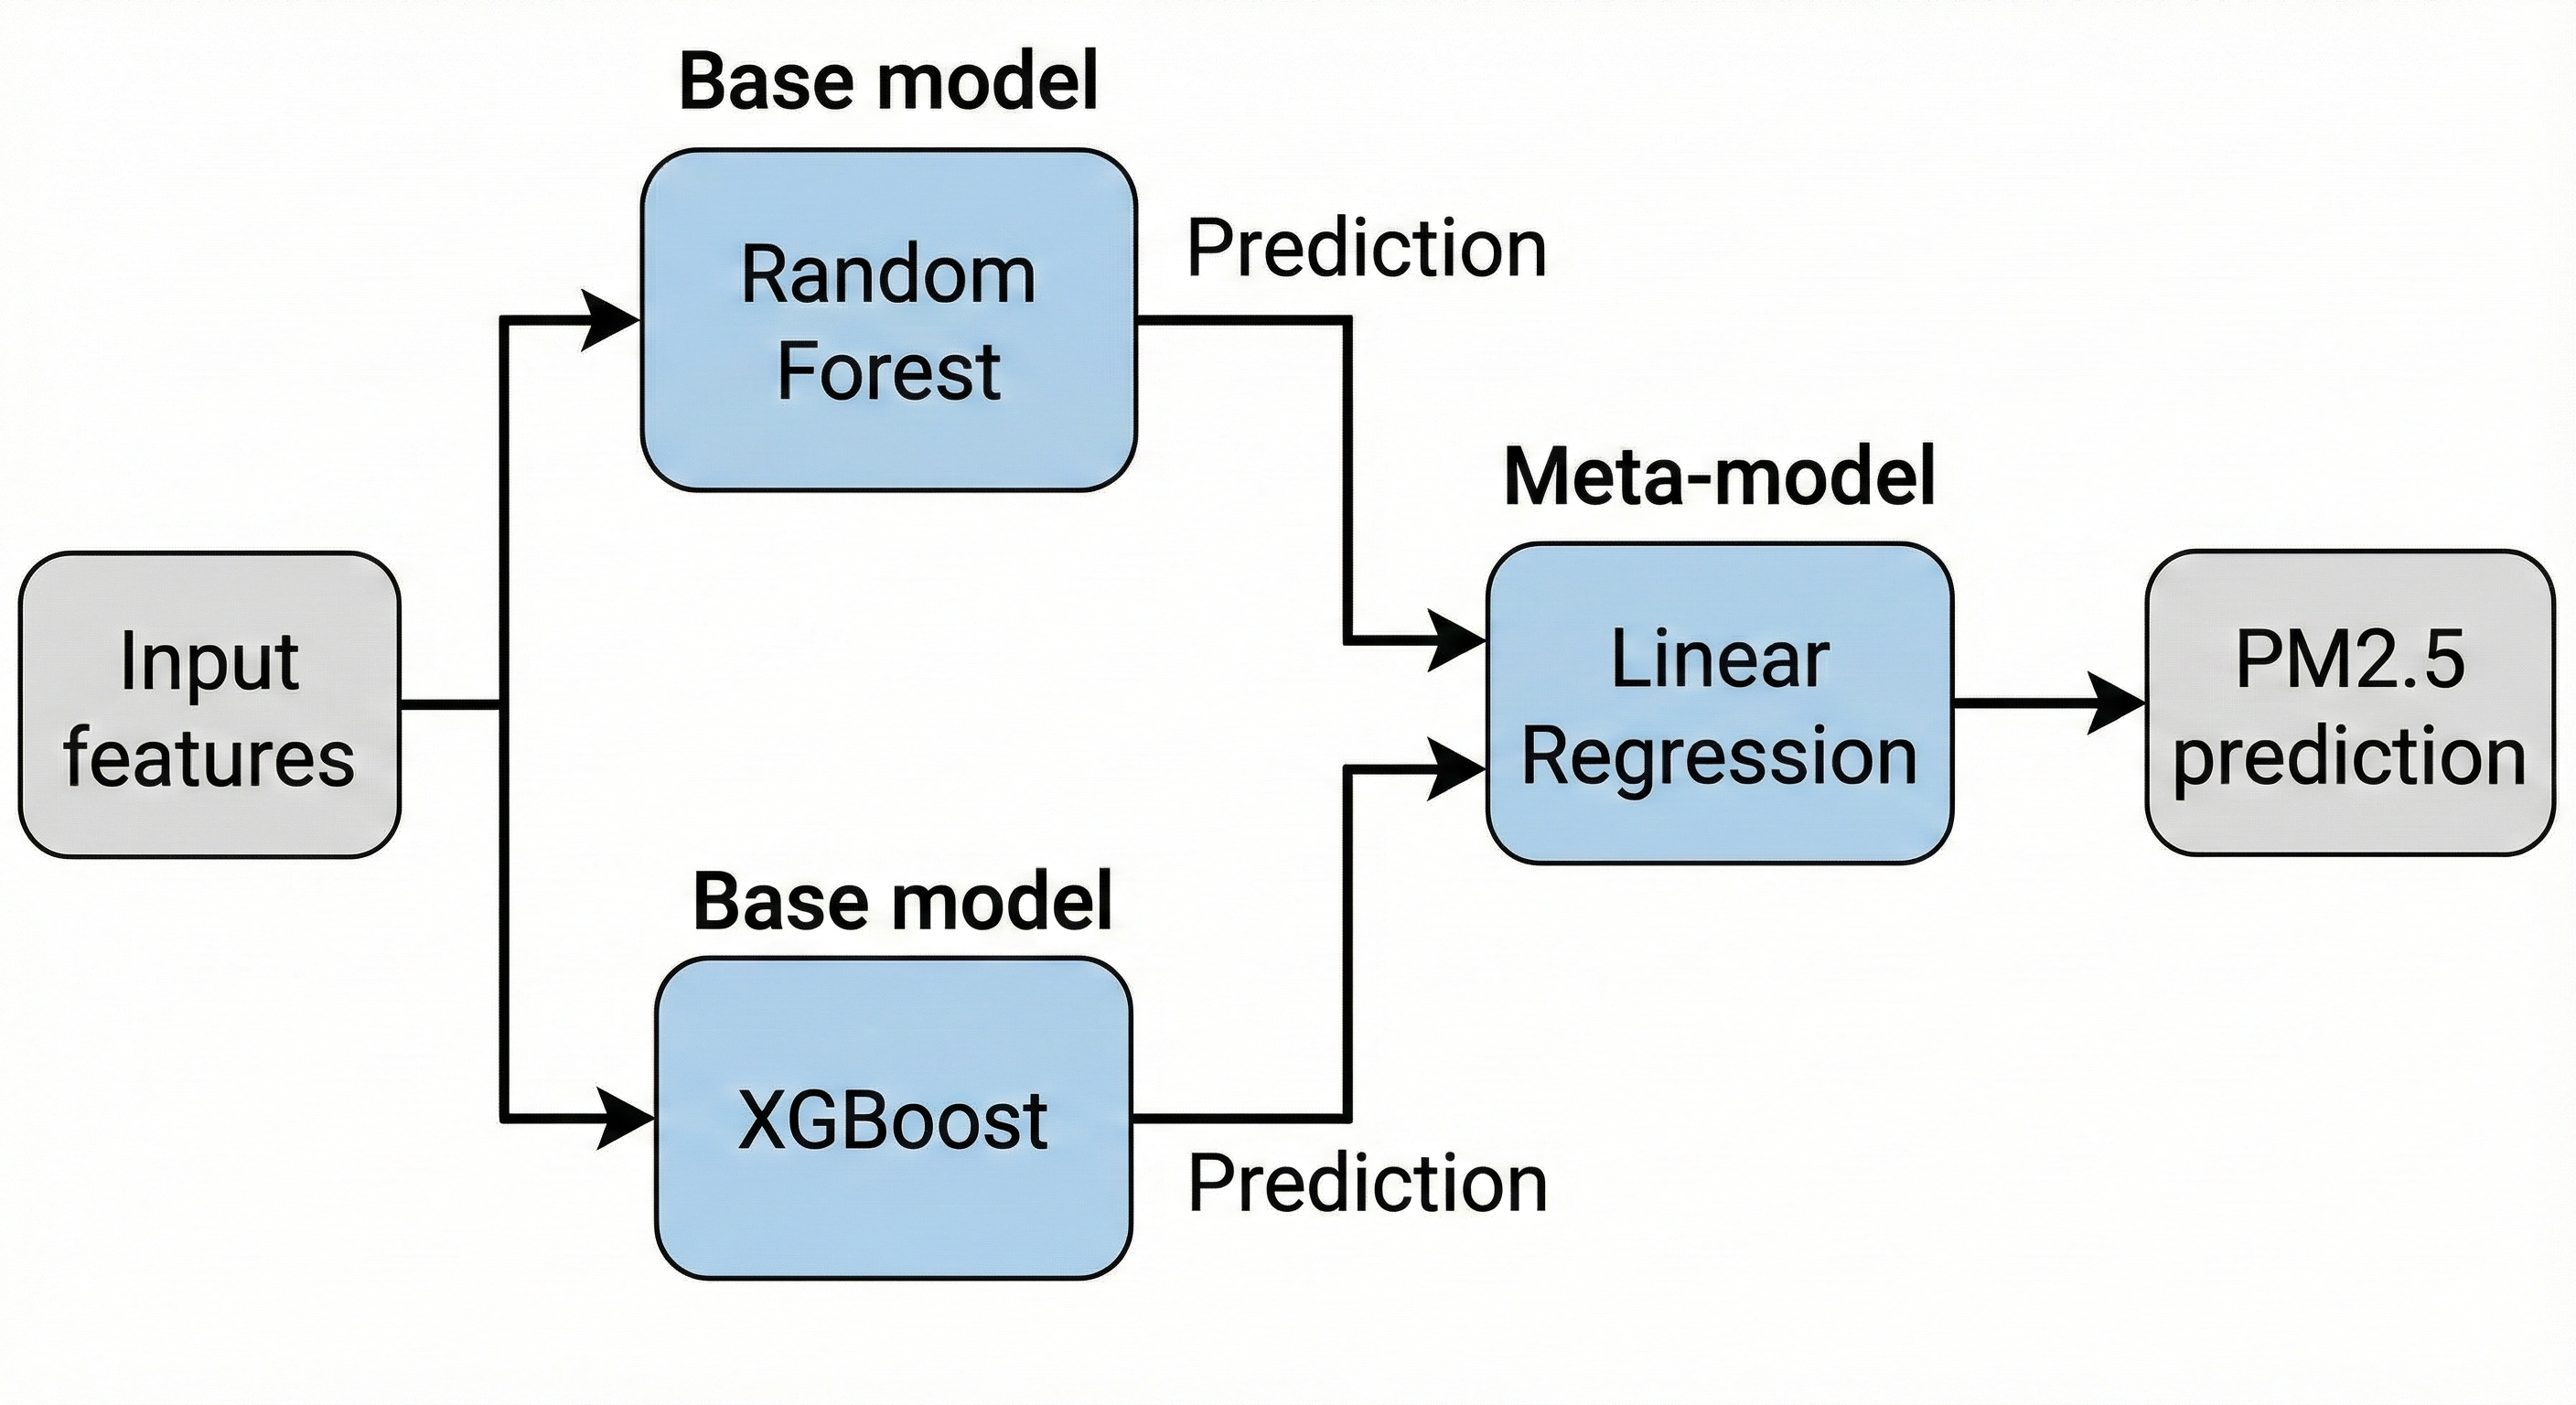
\includegraphics[width=0.9\textwidth]{Gemini_Generated_Image_rwtb7vrwtb7vrwtb.jpg}
    \caption{The proposed Stacked Generalization Ensemble architecture. Diverse base models (Random Forest and XGBoost) process the input features, and their predictions are fed into a Linear Regression meta-model to generate the final optimized PM2.5 prediction.}
    \label{fig:stacking_architecture}
\end{figure*}
% =======================================

\subsection{Data Sources and Collection}
The model development utilized a fused dataset combining ground-truth air quality measurements with corresponding satellite and meteorological variables.

\subsubsection{Ground-Truth Data}
The target variable for prediction is the \textbf{PM2.5 concentration} ($\mu g/m^3$). This data was sourced from a real-time air quality index dataset (CSV), serving as the ground truth for model training.

\subsubsection{Feature Data (Predictor Variables)}
The predictor variables were derived from a fused dataset that combines ground readings with data extracted from the \textbf{Google Earth Engine (GEE)} platform. The final feature set ($X$) includes six key variables: satellite data (Aerosol Optical Depth - AOD), meteorological data (Temperature, u-wind, v-wind), and geospatial data (Latitude and Longitude).

\subsection{Data Preprocessing}
Data preparation was performed to ensure model quality through several steps, including missing value handling, feature standardization of geospatial coordinates, and final cleaning. The complete data flow, from raw source acquisition through preprocessing to fusion, is illustrated in Fig. \ref{fig:data_pipeline}.

% === FIGURE 2: DATA PIPELINE ===
\begin{figure*}[htbp]
    \centering
    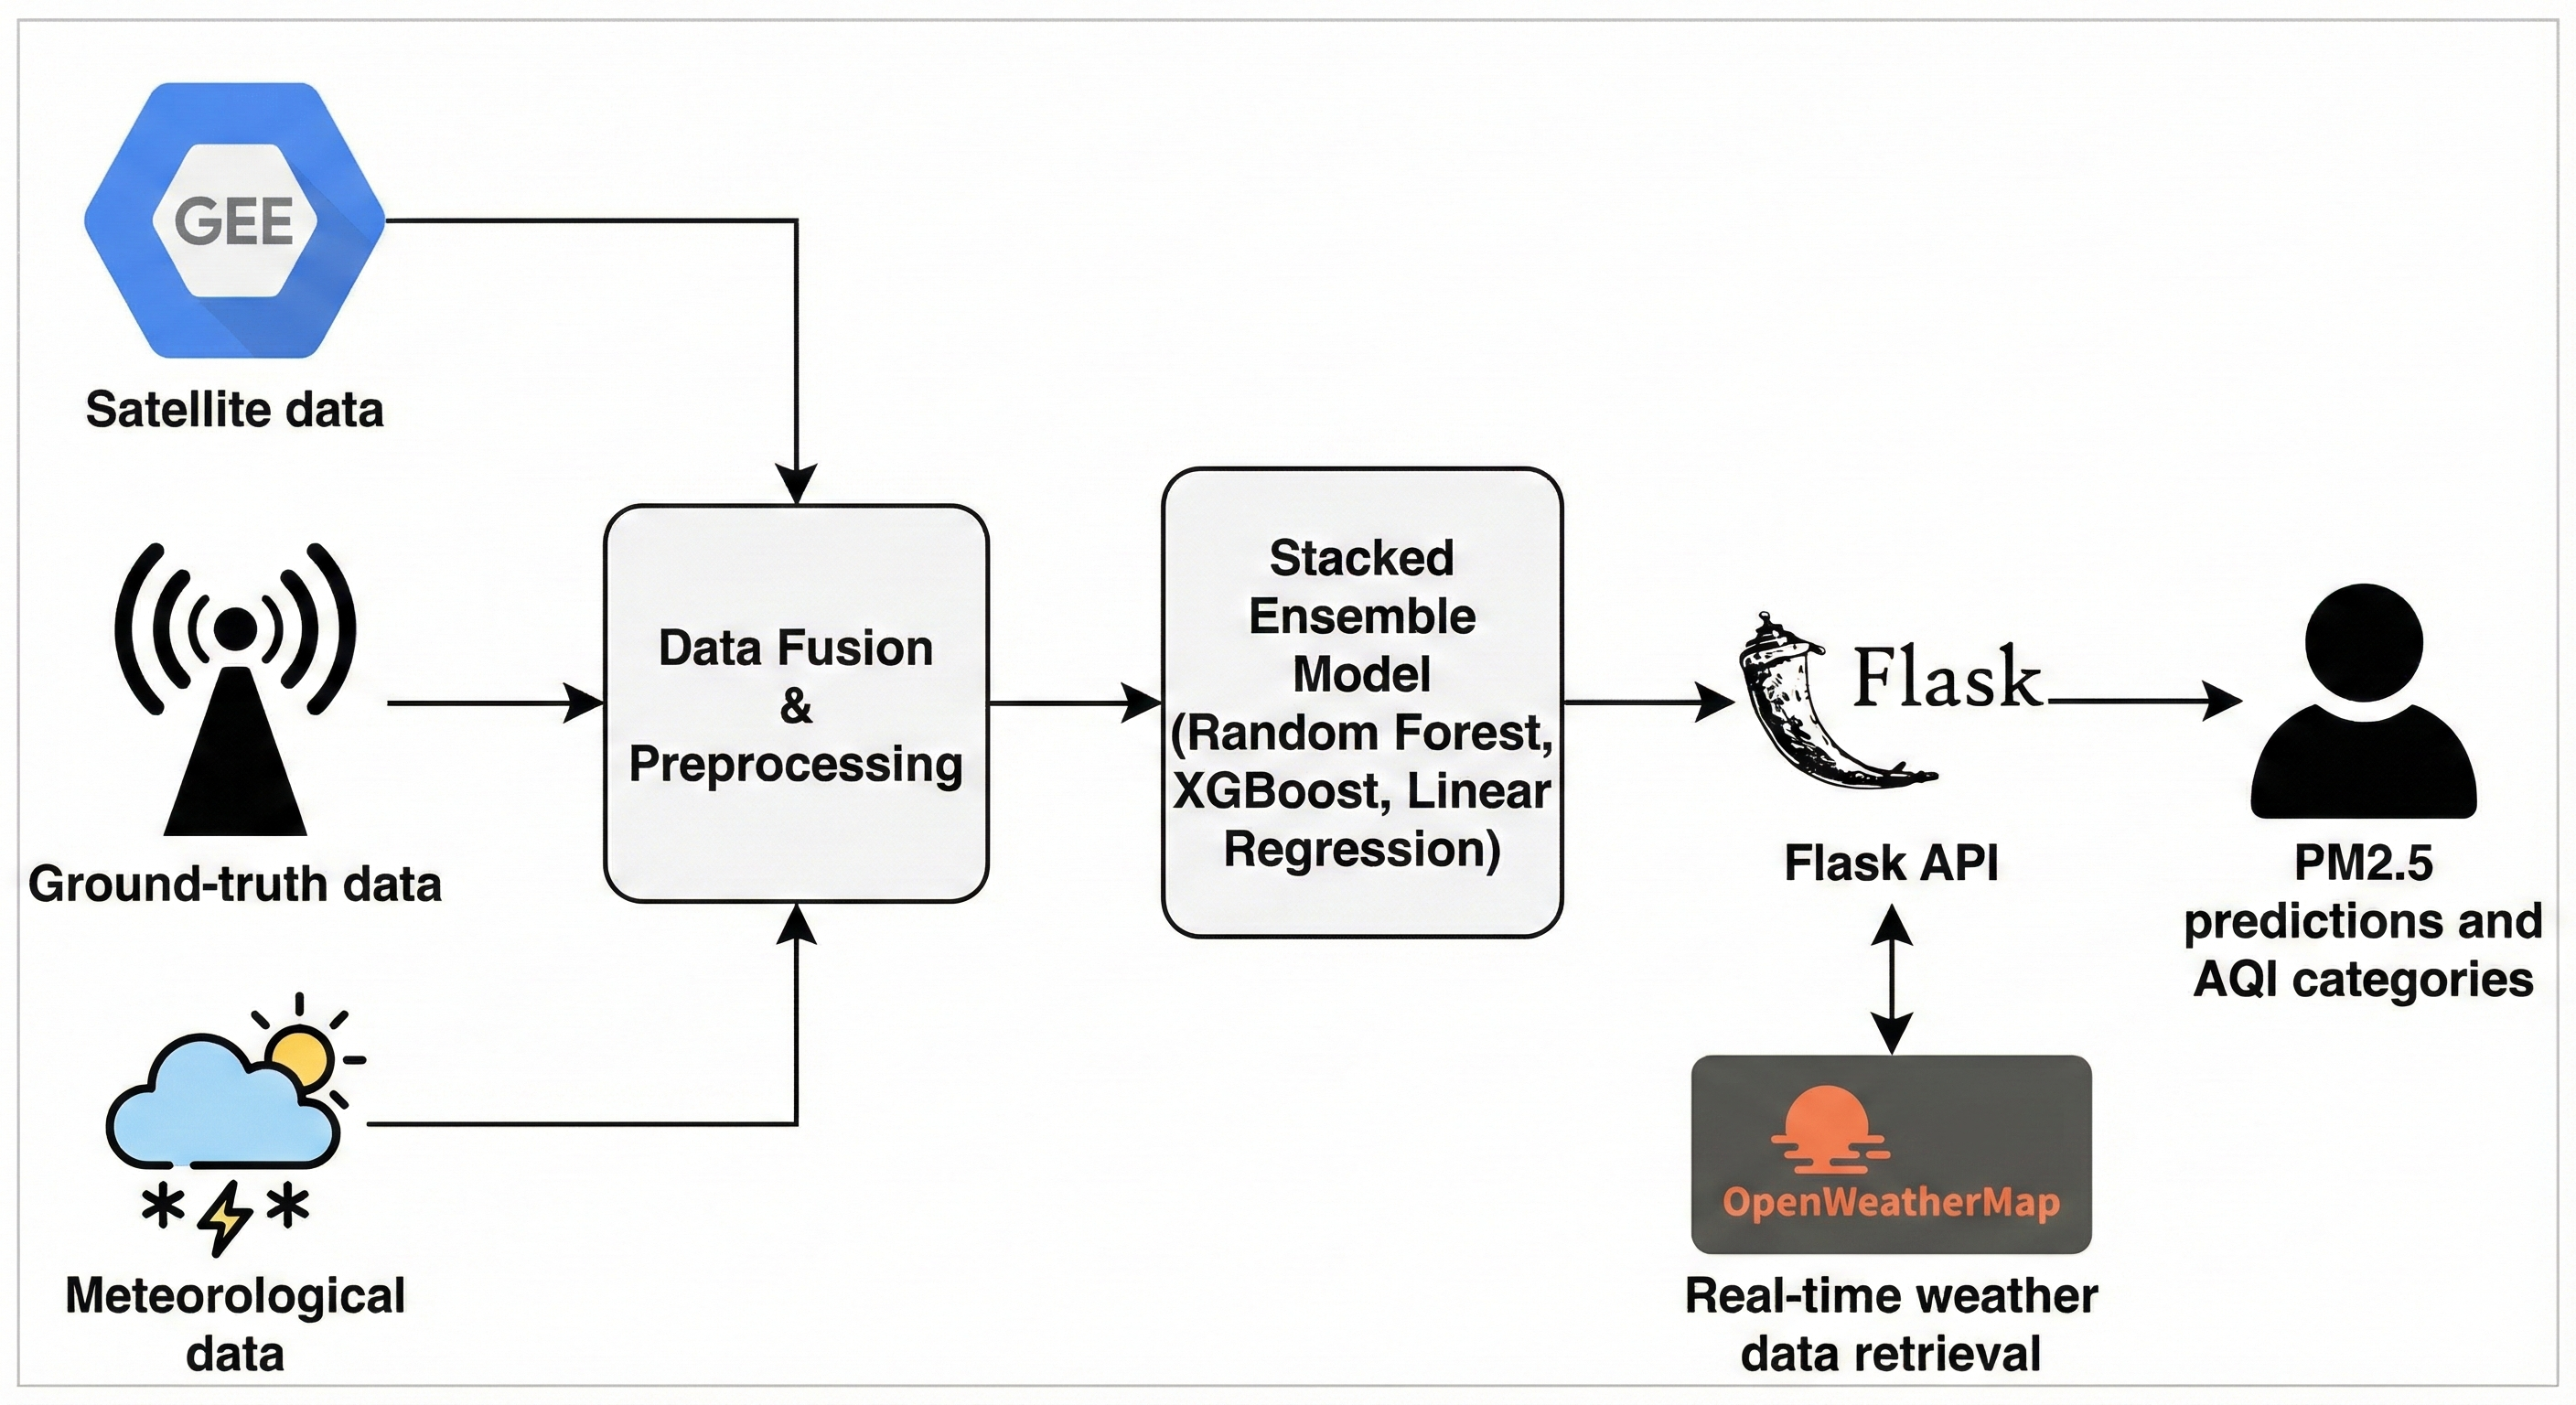
\includegraphics[width=0.9\textwidth]{Gemini_Generated_Image_fvuvsifvuvsifvuv.jpg}
    \caption{Comprehensive data processing pipeline illustrating the ingestion of heterogeneous data (satellite imagery, ground sensors, meteorology), followed by cleaning, feature extraction, and fusion into a unified dataset for model training.}
    \label{fig:data_pipeline}
\end{figure*}
% ===============================

\subsection{Model Training and Evaluation}

\subsubsection{Training Protocol}
The cleaned dataset was partitioned into a \textbf{training set (80\%)} and a \textbf{testing set (20\%)} using a random seed (`random\_state=42`) to ensure reproducibility.

The training process involved two stages: first, training the base models (RF and XGB) on the complete training feature set; second, generating predictions from these base models to serve as features for training the Linear Regression meta-model against the true target values.

\subsection{Comparative Results (Test Set)}
Model performance was evaluated on the held-out test set using \textbf{R-squared ($R^2$)} and \textbf{Root Mean Squared Error (RMSE)}. Table \ref{tab:results} summarizes the performance of the individual base models compared to the final stacked ensemble.

\begin{table}[htbp]
    \centering
    \caption{Comparative Performance Metrics on Test Set}
    \label{tab:results}
    % Using resizebox to ensure it fits column if needed,
    % though standard table usually fits fine.
    \resizebox{\linewidth}{!}{
    \begin{tabular}{lccc}
        \toprule
        \textbf{Model} & \textbf{R-squared ($R^2$)} & \textbf{RMSE ($\mu g/m^3$)} & \textbf{Role} \\
        \midrule
        Random Forest Regressor & 0.5367 & 65.54 & Base Model \\
        XGBoost Regressor & 0.4276 & 72.85 & Base Model \\
        \textbf{Stacked Ensemble Model} & \textbf{0.5592} & -- & \textbf{Final Model} \\
        \bottomrule
    \end{tabular}
    }
\end{table}

The \textbf{Stacked Ensemble Model} achieved the highest $R^2$ score of \textbf{0.5592}, outperforming the Random Forest ($0.5367$) and XGBoost ($0.4276$) base models.

\section{System Deployment Structure}
To operationalize the proposed methodology, the system is designed as an API endpoint capable of real-time inference. The practical workflow of this deployment is demonstrated in Fig. \ref{fig:deployment_structure}.

The deployment logic follows this sequence:
\begin{enumerate}
    \item \textbf{Input Collection:} The system accepts user-provided geospatial coordinates (Latitude, Longitude) and the current Aerosol Optical Depth (AOD).
    \item \textbf{Live Data Retrieval:} A real-time weather fetcher retrieves the necessary meteorological parameters from the OpenWeatherMap API.
    \item \textbf{Feature Integration:} Static inputs and dynamic weather data are aggregated into a single feature vector.
    \item \textbf{Stacked Prediction:} The feature vector is passed through the base models and then the meta-model to compute the final PM2.5 concentration.
    \item \textbf{Classification:} The predicted concentration is mapped to AQI categories and returned as a JSON response.
\end{enumerate}

% === FIGURE 3: DEPLOYMENT ===
\begin{figure*}[htbp]
    \centering
    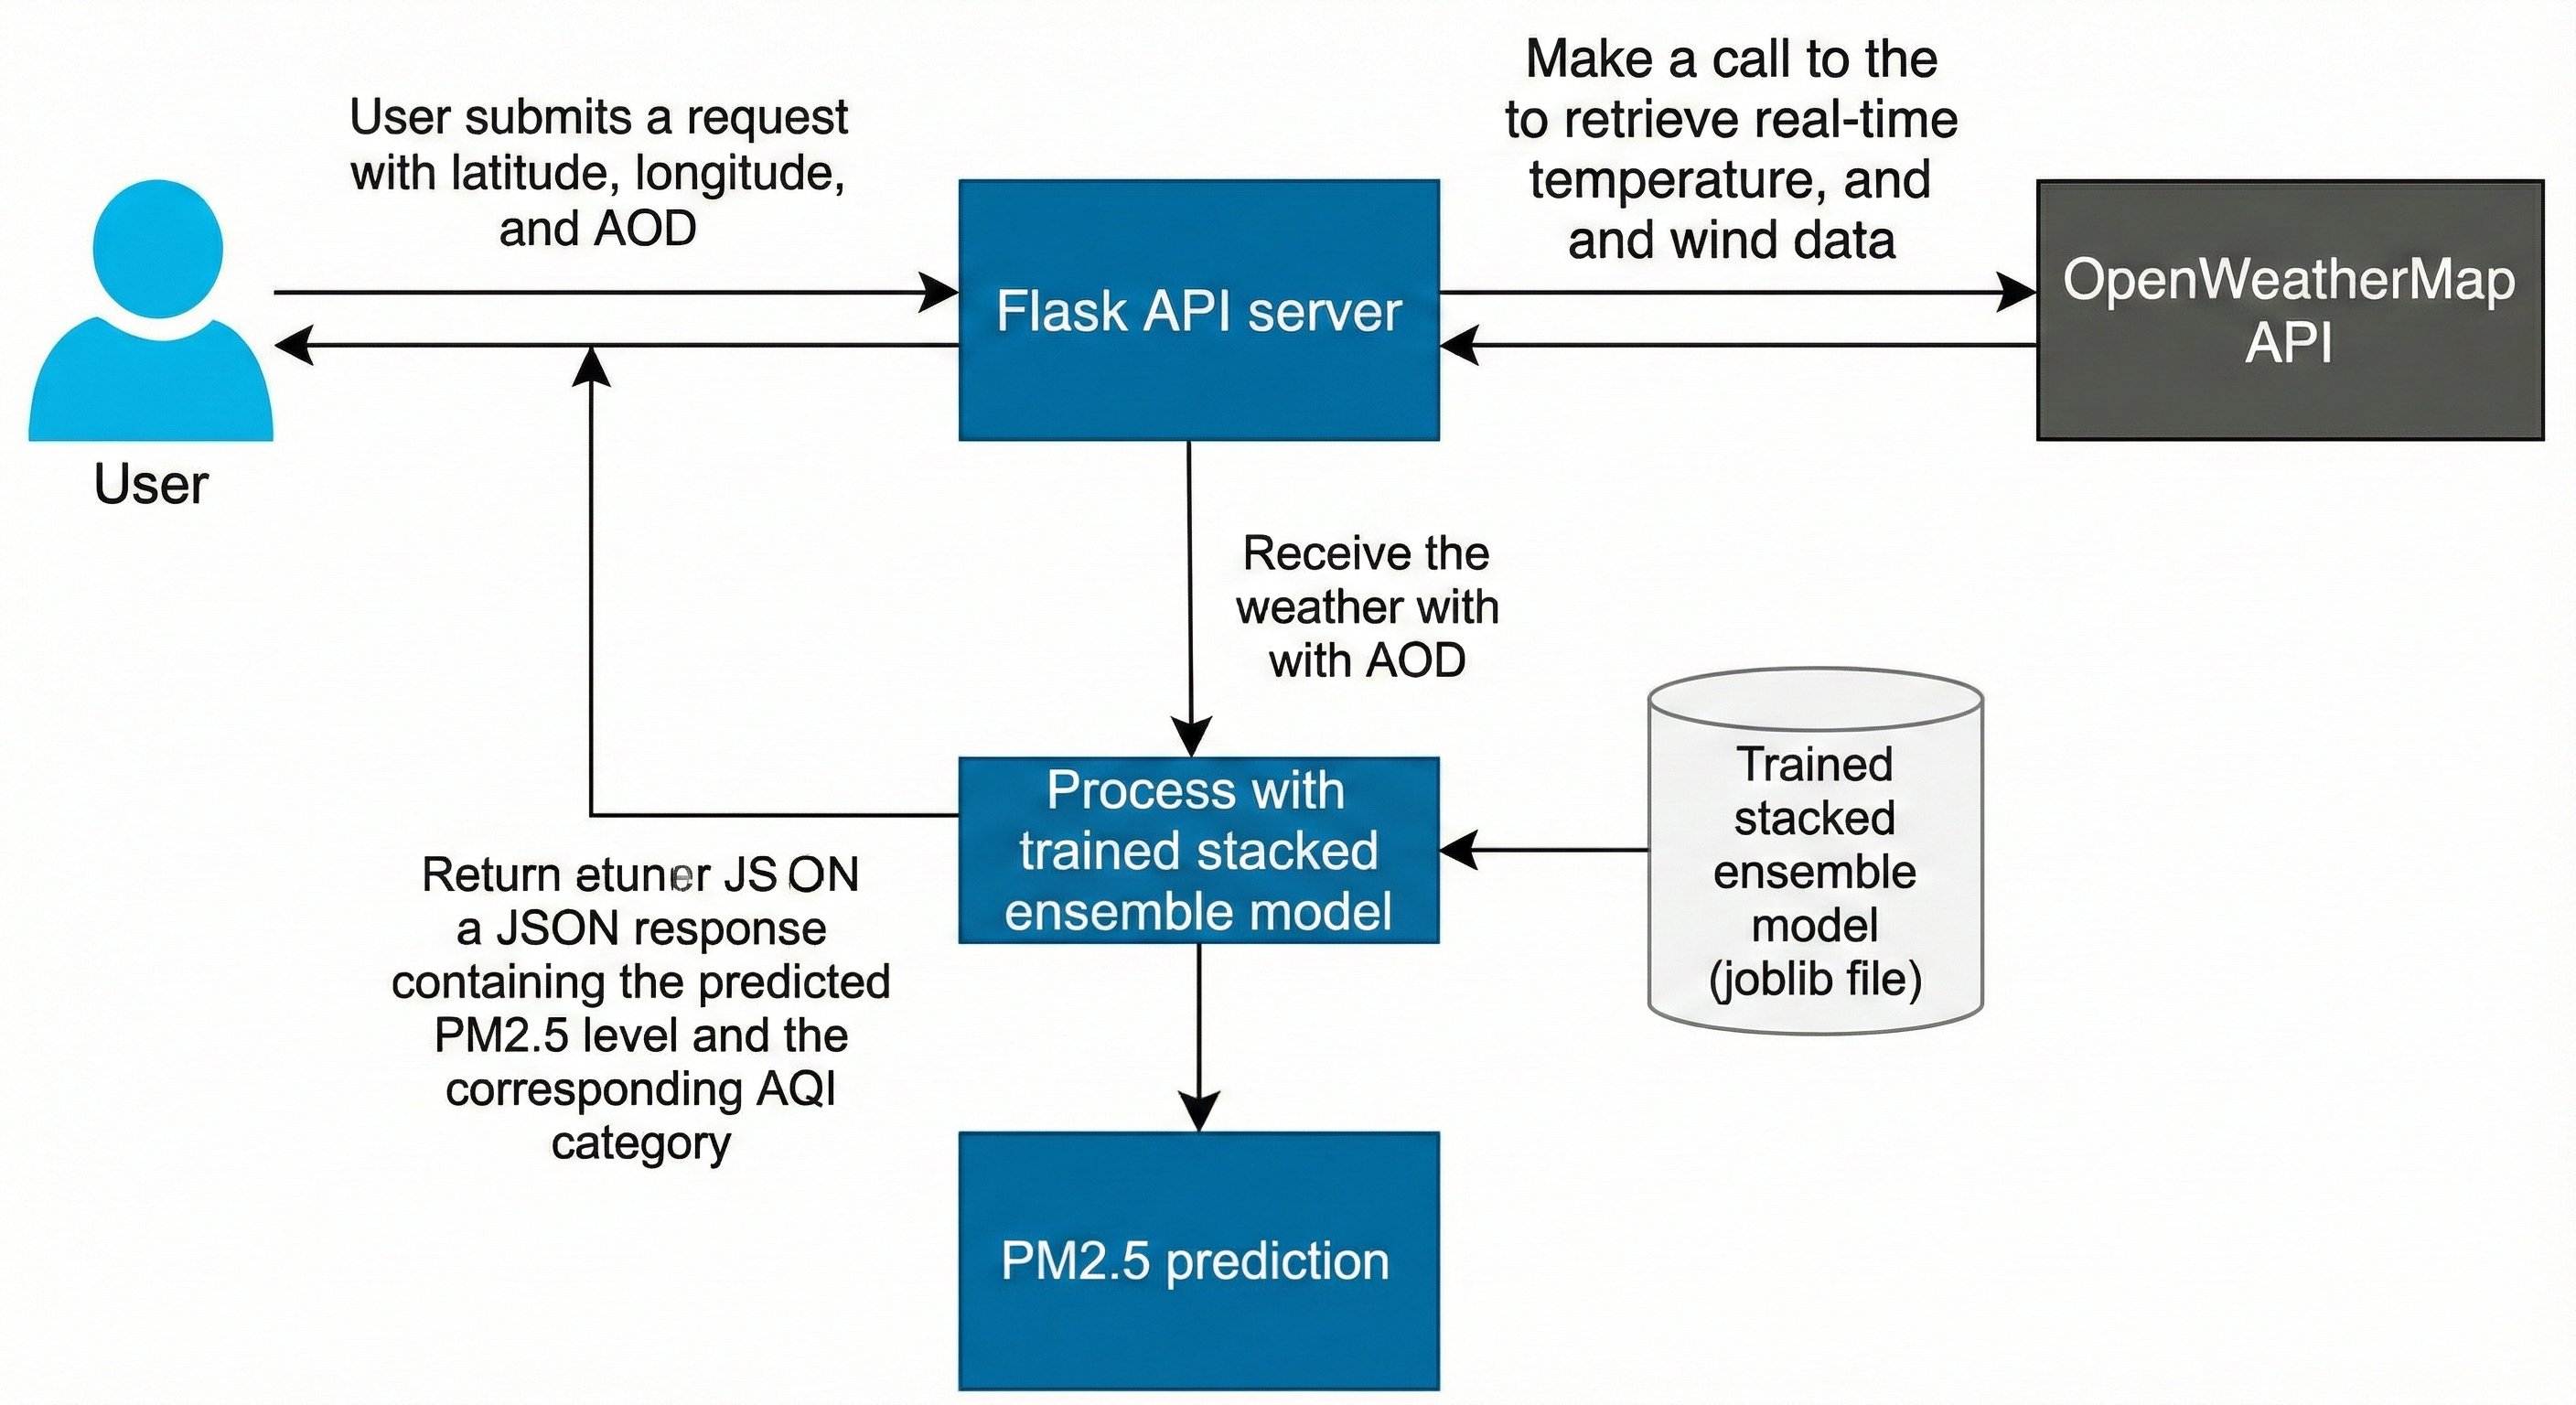
\includegraphics[width=0.9\textwidth]{Gemini_Generated_Image_r6lm2ir6lm2ir6lm.jpg}
    \caption{Operational system deployment structure. The system operates as an API that takes user location and AOD data, fetches real-time weather, runs the stacked prediction inference, and returns the PM2.5 value and AQI category as a JSON response.}
    \label{fig:deployment_structure}
\end{figure*}
% ============================

\section{Conclusion And Future Work}
% [Your Conclusion Text Here - Truncated for brevity]
\subsection{Conclusion}
This paper presented a robust machine learning framework... The key finding of this research is the superior predictive power of the Stacked Generalization Ensemble (SGE) model...

\subsection{Future Work}
% [Your Future Work Text Here - Truncated for brevity]
Building on the success of this heterogeneous data fusion...

\section*{Acknowledgment}
% [Your Acknowledgment Text Here]

% --- REFERENCES ---
% Ensure your bibliography is set up correctly here.
% For this example, I'm using the manual environment you provided previously.
\begin{thebibliography}{00}
\bibitem{b1}Méndez, M., et al. (2023). "Machine learning algorithms to forecast air quality: a survey." Artificial Intelligence Review 56(9): 10031-10066.
\bibitem{b2}Zhang, Z., et al. (2024). "A systematic survey of air quality prediction based on deep learning." Alexandria Engineering Journal 93: 128-141.
\bibitem{b3}Lee, J.-B., et al. (2022). "Development of a deep neural network for predicting 6 h average PM 2.5 concentrations up to 2 subsequent days using various training data." Geoscientific Model Development 15(9): 3797-3813.
% ... [Rest of your references] ...
\end{thebibliography}

\end{document}